\documentclass[12pt]{article}

\usepackage[left=2.5cm,right=2.5cm,top=2.5cm,bottom=2.5cm]{geometry}

\usepackage{amsmath}

\DeclareMathOperator{\trace}{trace}

\usepackage{graphicx}

\usepackage[font=small,labelfont=bf]{caption}

\usepackage{fancybox}

\usepackage{array}

\usepackage{multirow}

\usepackage[numbers,square,sort]{natbib}

\usepackage[resetlabels]{multibib}

\usepackage{hyperref}

\usepackage{comment}

\usepackage{makeidx}

\usepackage{amsfonts}

\usepackage{amssymb}

\usepackage{blindtext}

\usepackage{multicol}

\usepackage{enumitem}

\usepackage[mathscr]{euscript}

\setlength{\columnsep}{1cm}

\renewcommand{\labelenumii}{\arabic{enumi}.\arabic{enumii}}

\renewcommand{\labelenumiii}{\arabic{enumi}.\arabic{enumii}.\arabic{enumiii}}

\renewcommand{\labelenumiv}{\arabic{enumi}.\arabic{enumii}.\arabic{enumiii}.\arabic{enumiv}}

% Begin Narges's part__________________________________________________________

\title{Las Vegas randomized algorithms in distributed consensus problems}

\author{Narges Ghanei-610399155 \\Aaron Bateni-610399105\\Fateme Rashidi Shahri-610399131 }
\date{July 2022}

\begin{document}
	
	\maketitle
	\textbf{Abstract— We consider distributed consensus problems from the viewpoint of probabilistic algorithms. In particular, we provide an overview on some specific problems where randomization is critical in achieving consensus among multiple agents. Further, we show that the randomized algorithms which are used in this setting are the so-called Las Vegas randomized algorithms (e.g. \cite{bib24}). This class is different from that of Monte Carlo type, which has been recently successfully employed for various computationally difficult problems in systems and control. The objective of this paper is therefore to show the link between various distributed consensus problems and randomized algorithms for systems and control.}
	
		
		\tableofcontents
		\newpage
		
		\section{INTRODUCTION}
		In recent years, distributed consensus, agreement, and flocking problems have gained much attention in the systems and control community. Control theoretic approaches have proven to be useful in the analysis of distributed systems for specifications such as stability and agreement.Recent references include \cite{bib03}, \cite{bib04}, \cite{bib06}, \cite{bib07}, \cite{bib10}, \cite{bib12}, \cite{bib16}, \cite{bib18}, \cite{bib20}, \cite{bib21}, \cite{bib25}, \cite{bib27}.
		For additional details, we refer to \cite{bib05} which gives a summary of the development of such problems along with some new results and to the special issue \cite{bib01} which describes current research on this topic.
		\par
		In particular, we consider the average consensus problems, which can be described as follows: There is a set of $N$ agents that possess numerical values and communicate their values with their neighbors in an iterative way. The goal is that all agents eventually reach a common value, which is the average of the initial values of all agents. Such problems arise in applications related to multi-vehicle coordination, load balancing, and sensor networks. 
		\par
		The objective of this paper is to present the average consensus problems from the unifying viewpoint of probabilistic and Las Vegas algorithms. Recently, in the field of systems and control, techniques based on randomized algorithms have been developed (see, e.g, \cite{bib23}, \cite{bib26}); however, we will see how the classes of algorithms there and those in the consensus problems perform differently. According to a formal definition used in computer science \cite{bib17}, a randomized algorithm is an algorithm that makes random choices during its execution to produce a result. This implies that even for the same input, the algorithm might produce different results at different runs, and moreover the results may even be incorrect.
		\par
		More specifically, in this paper, we aim at clarifying two points: One is to introduce randomized algorithms appearing in several variations of average consensus problems. Such techniques are shown to be useful and can be crucial. Indeed, in some cases, there are even stronger results implying that no deterministic method can efficiently achieve consensus \cite{bib09}, \cite{bib17}. The other is to show the difference in the classes of algorithms appearing in consensus problems and those in the probabilistic approach in control. To this end, we provide an overview on the probabilistic approach in control and see that the main algorithms there are the Monte Carlo type. Then, we show that the algorithms in the average consensus belong to the class of Las Vegas type algorithms. This class has recently been exploited for problems related to systems and control \cite{bib11}, \cite{bib24}.
		\par
		The paper is organized as follows. In Section 2, we present a general robustness analysis problem. In Section 3, randomized algorithms of Monte Carlo type for such problems are discussed. In Section 4, we provide an introduction to Las Vegas algorithms. In Section 5, we discuss three cases of average consensus problems and show the importance of probabilistic techniques. We conclude the paper in Section 6.
		\par
		

		\section{PROBABILISTIC APPROACH TO UNCERTAIN SYSTEMS}
		In the past decade, probabilistic methods for systems and control have significantly progressed. This research has been also motivated by results showing that many problems naturally arising in control are computationally difficult and are in fact NP-hard. Such problems can be found in areas including uncertain and hybrid systems. The development and application of probabilistic techniques to analysis and synthesis control problems have been proven effective yielding computationally efficient algorithms. For a detailed account on this topic, we refer to \cite{bib23}, \cite{bib26}.
		\par
		In this section, we introduce a robustness analysis problem  where various uncertainties can be represented. Given a system containing uncertain components, the objective of robustness analysis is to find whether certain control properties hold for all uncertainties. This general problem can be formulated as follows.
		\par
		We first assume that the uncertainty in the system is represented by a real/complex matrix $\Delta$ and further that $\Delta$ belongs to a bounded set $\mathscr{B}$. On the other hand, the system property is measured by the performance function $J : \mathscr{B} \rightarrow \mathbb{R}$. The function $J$ is assumed  to be a measurable function. A general robustness analysis problem is to check whether a certain performance level $\gamma$ is guaranteed for all possible uncertainties $\Delta \in \mathscr{B}$. In other words,  we are interested in finding if 
		\begin{equation}
			\label{eqn:1}
			J(\Delta ) \leqslant \gamma \textrm{ for all } \Delta \in \mathscr{B}
		\end{equation}
		\par
		If the uncertainty $\Delta$ is of general form, there are barriers in terms of computational complexity for solving this problem. We follow a probabilistic approach and shift the meaning of robustness from the deterministic sense as in \ref{eqn:1} to a probabilistic one.
		\par
		In the probabilistic approach, we assume that the uncertainty matrix $\Delta \in \mathscr{B}$ is a random matrix; here, random variables are denoted in boldface letters. Let $Prob_{\Delta}(.)$ be the corresponding probability measure associated to $\Delta$.
		\par
		We consider two specific performance criteria using $J(\Delta )$. The first is the worst-case performance defined by 
		\begin{equation} 	
			J_{max}:= \sup_{\Delta \in \mathscr{B} }J(\Delta ) 
		\end{equation}
		The other is the average-case performance 
		\begin{equation*} 	
			J_{ave}:= E_{\Delta}(J(\Delta )) 
		\end{equation*}
		where $E_{\Delta}(J(\Delta ))$ denotes the expected value of the performance function with respect to the uncertainty set $\mathscr{B}$.
		\par
		A performance function commonly employed in robustness  analysis is the $H^{\infty }$ norm of a closed-loop system. In this case, let the function $J(\Delta)$ be the norm of the system from the disturbance to the controlled output. Depending on the criterion of interest, we may choose to work with the worst-case performance or the average-case performance.
		\par
		In this setting, a decision problem refers to a situation whose answer to an instance is either yes or no. Here, we address two uncertain decision problems: For a given performance level $\gamma > 0$, check if $J_{max} \leq \gamma $ and $J_{ave} \leq \gamma$ . We next show that these problems can be efficiently solved in a probabilistic sense.
		
		
		\section{MONTE CARLO RANDOMIZED ALGORITHMS}
		We now introduce Monte Carlo randomized algorithms. Most probabilistic results derived in systems and control are based on this type of algorithms. We will see later that this class is different from the one appearing in consensus problems. The definition is as follows \cite{bib17}.
		\par
		
		\textit{Definition 1: A Monte Carlo randomized algorithm (MCRA)} is a randomized algorithm that may produce a result that is incorrect (in the deterministic sense), but the probability of such an incorrect result is bounded.
		\par
		In general, for an MCRA, the results and the running times would be different from one run to another since the algorithm is based on random sampling. As a consequence, the computational performance of such algorithms is usually measured by their 
		\textit{expected} running times. An MCRA is said to be 
		\textit{efficient} if the expected running time is of polynomial order in the problem size.
		For decision problems, MCRAs can be divided into two classes based on how the error of the outputs are evaluated.
		\par
		An MCRA for a decision problem is said to have onesided 
		\textit{error} if it always provides a correct solution in one of the possible instances, but may provide a wrong solution for the other one \cite{bib17}.
		\par
		
		\begin{center}
			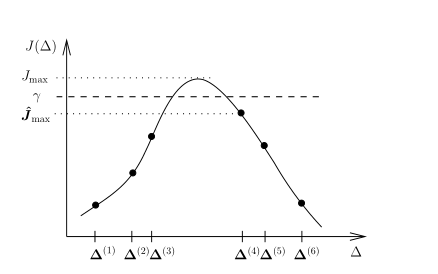
\includegraphics[width=0.49\linewidth]{1.png}
			\captionof{figure}{One-sided MCRA: The worst-case performance when $\hat{J}_{max}<\gamma < J_{max}$}
		\end{center}
		
		
		The MCRA for the worst-case performance belongs to this class. This algorithm involves the computation of the empirical maximum, which is defined by 
		\begin{equation*} 	
			\hat{J}_{max}:= \max_{i=1, 2, ..., N}J(\Delta ^{(i)}) 
		\end{equation*}
		where $
		\Delta (i) \in \mathscr{B} , i=1,2,...,N$, are independent and identically distributed (i.i.d.) samples of the random uncertainty matrix $\Delta$ generated according to the probability measure $Prob_{\Delta }$. Notice that the empirical maximum $\hat{J}_{max}$ is a random variable itself since its value depends on the random samples chosen for its computation. Fig. 1 shows a plot of $J(\Delta)$ and illustrates the concept for this problem. This algorithm is a one-sided MCRA in the following sense. For a given performance level $\gamma > 0$, if $J_{max}\leq \gamma $, then clearly the probability that the algorithm outputs the correct answer is one. Hence, this algorithm always provides a correct solution for this instance. On the other hand, if $J_{max}>
		\gamma $, then the probability of obtaining $\hat{J}_{max}\leq\gamma $ is nonzero. This implies that, for this instance, the algorithm can give an erroneous result with a nonzero probability.
		\par
		Now, noticing that the empirical maximum $\hat{J}_{max}$ is always smaller than $J_{max}$, we shall pose a natural question, how well does $\hat{J}_{max}$ estimate the true maximum? Under a sufficiently large sample size N, a probabilistic statement can be made; see, e.g., \cite{bib22}, \cite{bib23}.
		\par
		Another class of MCRAs for decision problems is that of 
		\textit{two-sided error} algorithms. Such algorithms may produce a wrong solution for both instances when the answer is yes and no \cite{bib17}. The average-case problem is an example of a two-sided MCRA; for details, we refer to \cite{bib24}.
		
		
		\section{LAS VEGAS RANDOMIZED ALGORITHMS}
		We introduce the Las Vegas algorithms and its basic properties. This type has not been employed much in the context of control, but is important for consensus problems.
		\par
		
		
		\subsection{Preliminaries}
			The formal definition is given in \cite{bib17} as follows: 	
			\textit{Definition 2: Las Vegas randomized algorithms (LVRA)} 	are randomized algorithms which always give the correct answer. The only difference from one run to another is the 	running time.
% End Narges's part__________________________________________________________			
% Begin Aaron's part__________________________________________________________
			For obvious reasons, such algorithms are also called \emph{zero-sided error} Monte Carlo. Because of randomization, the running time is random (similarly to MCRA) and may be different in each execution. Hence, the expected running time is of interest. We note that the expectation is with respect to the random samples generated during each run and not to the input of the algorithm. Furthermore, if the expected running time is of polynomial order in the problem size, the algorithm is said to be \emph{efficient}.
			\par
			A well-known example is the \textit{Randomized Quick Sort (RQS)} \cite{bib14}, \cite{bib17} described in the following.
			\par
			\textit{Example 1:} Given a set 
			
			\begin{equation*}
				\mathscr{S}_1 = {x_1 , . . . , x_N } 
			\end{equation*}
			
			of $N$ real numbers, consider the problem of sorting the numbers in an increasing order. The RQS is a randomized algorithm that solves this problem in a computationally efficient way. The outline of the algorithm is as follows
			\begin{itemize}
				\item[1]
				Randomly select a number $x^{(1)}$ in the set $\mathscr{S}_1$.
				\item[2]
				Perform deterministic comparisons between $x^{(1)}$ and other elements in $\mathscr{S}_1$ . Let $\mathscr{S}^{(2)}$ be the set of numbers smaller than $x^{(1)}$ , and let $\mathscr{S}^{(3)}$ be the set of numbers larger than $x^{(1)}$.
				\item[3]
				Recursively apply the two steps above to the sets $\mathscr{S}^{(2)}$ and $\mathscr{S}^{(3)}$. Output the sorted version of $\mathscr{S}^{(2)}$, $x^{(1)}$, and then the sorted version of $\mathscr{S}^{(3)}$.
			\end{itemize}
			\par
			The rationale for randomization in 1 is as follows: The algorithm would be most efficient if the original set $\mathscr{S}_1$ is divided into two sets having the same cardinalities. However, this requires the median of $\mathscr{S}_1$ as $x^{(1)}$ , which is costly to find. To randomly choose $x^{(1)}$ is a simple strategy, but on average provides a good estimate of the median.
			\par
			In a formal analysis, the running time is measured by the number of comparisons. It follows that the expected running time is of order $O$($N$log$N$); in fact, the running time is of this order with high probability, at least $1 − 1/N$ \cite{bib15}. The \textbf{RQS} is more efficient than, for example, a deterministic brute-force approach, which has complexity $O$($N^2$). 
			\par
			For the \textbf{RQS}, the worst case is when the randomly chosen number in $1$ always happens to be either the smallest or the largest in the set. Then, the running time achieves the order $O$($N^2$). The \textbf{RQS} is, however, recognized as one of the most useful general purpose sorting algorithms \cite{bib14}. $\triangledown$
			\par
			As mentioned above, Las Vegas algorithms are randomized algorithms that always produce correct results. It is clear that this feature can be expected for only a limited number of Monte Carlo type algorithms. Hence, their application is naturally limited. One such algorithm is developed for a switched systems problem in \cite{bib11}.
			\par
		\subsection{LVRAs for uncertain decision problems}
			We now present a discussion parallel to that on uncertain systems in Sections 2 and 3 for Las Vegas algorithms.
			\par
			First, as the uncertainty set, we take a finite subset $\tilde{\mathscr{B}}$ of $\mathscr{B}$ with $N$ elements given as
			\begin{equation*}
				\tilde{\mathscr{B}} = \left\{\tilde{\Delta}_1, \tilde{\Delta}_2, ..., \tilde{\Delta}_N\right\} \subset \mathscr{B}
			\end{equation*}

			\begin{center}
				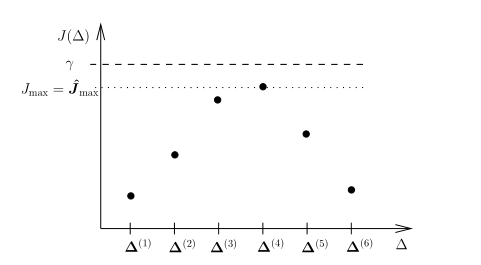
\includegraphics[width=0.49\linewidth]{2.png}
				\captionof{figure}{LVRA: The worst-case performance when $J_{max} = \hat{J}_{max} < \gamma$}
			\end{center}
			
 
			
			Assuming that the uncertain matrices in $\tilde{\mathscr{B}}$ are random variables, we consider a discrete probability measure; as in Section II, this measure is denoted by Prob$_\Delta$. Similarly, let the performance function be $J : \tilde{\mathscr{B}} → \mathbb{R}$. The general robustness analysis problem is to find whether, for a given performance level $\gamma > 0$, $J(\Delta) \leq \gamma$ for all $\Delta \in \tilde{\mathscr{B}}$. The corresponding worst-case performance is
			\begin{equation}
				J_{max} := \max_{\Delta \in \tilde{\mathscr{B}}}J(\Delta)
			\end{equation}
			and the average case performance is
			\begin{equation*}
				J_{ave} := E_\Delta\left[J(\Delta)\right] = \sum_{i=1}^N J(\tilde{\Delta}_i)Prob_\Delta(\tilde{\Delta}_i)
			\end{equation*}
			We now consider the uncertain decision problem for the worst-case performance. Given a scalar $\gamma > 0$, check whether $J_max \leq \gamma$. The LVRA for this case is as follows: Let $\tilde{\mathscr{B}}_0 = \tilde{\mathscr{B}}$ and let $k = 1$. Also, let $\bar{J}^{(0)} = -\inf$. At the $k$th step, randomly select a sample $\Delta^{(k)}$ from $\tilde{\mathscr{B}}_{k-1}$. Then, set $\bar{J}^{(k)} = max \left\{J(\Delta^{(k)}), \bar{J}^{(k-1)}\right\}$ and $\tilde{\mathscr{B}}_k = \tilde{\mathscr{B}}_{k-1} \ {\Delta^{(k)}}$, and go to the next step. After the $N$th step, the maximum performance over the samples is given by $\hat{J}_{max} = \bar{J}^{(N)}$.
			\par
			This algorithm always outputs the correct answer and hence is a Las Vegas type. For either problem instance $(J_{max} \leq \gamma$ or $J_{max} > \gamma)$, the value \textbf{$\hat{J}_{max}$} that the algorithm produces coincides with the true value $J_{max}$. This is illustrated in Fig. 2.
			\par
			When $N$ is large, the computational complexity can be relaxed by modifying the algorithm just described. The resulting algorithm is a Monte Carlo type. This can be done by stopping at the $k$th step with $k < N$ and by computing the maximum performance over the $k$ samples. In fact, the resulting algorithm becomes a one-sided MCRA. We remark that this approach is closely related to the ordinal optimization; see, e.g., \cite{bib08}. The objective there is to find not the maximum performance value but the value that is at least within the $m$th largest.
			\par
			The average-case performance can be similarly discussed.			
			
	\section{LAS VEGAS RANDOMIZED ALGORITHMS FOR DISTRIBUTED AVERAGE CONSENSUS}
		In this section, we present several problems in distributed average consensus where the application of Las Vegas type algorithms can be effective and sometimes in fact crucial.
		
		\subsection{\textit{General problem setup}}
			Consider a network of $N$ nodes specified by the graph ($\mathscr{V}$, $\mathscr{E}$), where $\mathscr{V} := {1, 2, . . . , N }$ is the set of nodes and $\mathscr{E}$ is the set of edges. The graph is assumed to be undirected and connected (see, e.g., \cite{bib17} for an introduction to random graph theory); this means that the edges are not associated with directions and that for any $i, j \in \mathscr{V}$, there is a path that connects the nodes $i$ and $j$. At time $k$, each node $i$ has a scalar value $x_i(k)$ whose initial value is $x_i(0)$.
			\par
			The goal is to provide an algorithm such that (i) the nodes update their values $x_i(k)$ using the information communicated from their neighbors and (ii) the values of the nodes eventually converge to the average of the initial values. To this end, for a consensus algorithm, there are two elements that need to be determined: The rules for the nodes to update their values and the neighbors with which each node should communicate. 
			\par
			This problem is a particular version of distributed consensus. In general, consensus problems do not require to which number the values of the nodes must converge, but only that the number should be the same for all nodes. In the following, we consider three cases of this problem. The difference is in the range of the node values: Real numbers, integer (quantized) numbers, and binary numbers. 
			\par
			We introduce some notation that will be used throughout this section. Let the $N$-dimensional vector consisting of all node values at time $k$ be $x(k) = [x_1(k) \hdots x_N(k)]^T$. The communication pattern for the nodes at time $k$ is specified by the edge set $\tilde{\mathscr{E}}(k) \subset \mathscr{E}$, i.e., if $\{i, j\} \in \tilde{\mathscr{E}}$, then $x_i(k)$ is updated using $x_j(k)$ and vice versa; in this case, the nodes $i$ and $j$ are \emph{neighbors} of each other at this time. In general, neighbors of a node may change over the time.
		\subsection{\textit{Real-valued case}}
			We first present the case when the node values take real numbers which is studied in \cite{bib28}. We say that average consensus (in a deterministic sense) is achieved if the following condition is satisfied:
			\begin{equation}
				\lim_{k \rightarrow \inf} x_i(k) = \frac{1}{N} \sum_{j=1}^{N} x_j(0) \text{ for all } i = 1, ..., N.
			\end{equation}
			The update rule for the node $i$ takes a linear form as
			\begin{equation}
				x_i(k+1)=W_{ii}(k) x_i(k) + \sum_{j \in \mathscr{N}_i(k)} W_{ij}(k) x_j(k),
			\end{equation}
			where $\mathscr{N}_i(k) := \{j : \{i, j\} \in \tilde{\mathscr{E}}(k)\}$ is the set of neighbors for node $i$ at time $k$, and $W_{ij}(k)$ are the weights. The weights are time varying and are specified by
			\begin{equation}
				W_{ij}(k)=\begin{cases}
					\frac{1}{1+max\{d_{i}(k),d_{j}(k)\}} & \text{if }\{i,j\}\in \ensuremath{\tilde{\mathscr{E}}(k),}\\
					1-\sum_{l\in\mathscr{N}_{i}(k)}W_{il}(k) & \text{if }i=j\\
					0 & \text{otherwise,}
				\end{cases}
			\end{equation}
			where $d_i(k)$ denotes the cardinality of $\mathscr{N}_i(k)$, that is, the number of neighbors for the node $i$. Notice that the sum of the weights at each node is one; this makes the matrix $W$ a stochastic one. In \cite{bib28}, it is remarked that the weights $Wij(k)$ in (6) are adopted from the Metropolis algorithm used in Markov chain Monte Carlo. 
			\par
			The update rule in (5) can be implemented in a distributed and causal manner. This is because the nodes only require the information of the values coming from their neighbors at the time. Regarding the communication pattern specified by $\tilde{\mathscr{E}}(k)$, $k \in \mathbb{Z}_+$, the assumption is as follows: The graph ($\mathscr{V}$, $\bigcup_{s \geq k} \tilde{\mathscr{E}}(s)$) is a connected graph for all $k$. In words, this says that the collection of edge sets occurring infinitely often over the time makes it a connected graph. 
			\par
			The following is the main result of \cite{bib28}.
			\par
			\textit{Theorem 1:} Under the update rule in (5) and the communication pattern satisfying the condition that the graph ($\mathscr{V}$, $\bigcup_{s \geq k} \tilde{\mathscr{E}}(s)$) is a connected graph for all $k$, distributed average consensus in the sense of (4) is achieved for each initial condition $x(0) \in \mathbb{R}^N$. 
			\par
			This theorem provides a condition on $\tilde{\mathscr{E}}(k)$ which must be specified at the time of implementation for the average consensus in a deterministic sense. Similar conditions are employed in other schemes in, e.g., \cite{bib05}, \cite{bib12}, \cite{bib16}. 
			\par
			A simple way to implement a communication pattern with the desired property is to employ randomization: Each node $i$ communicates with a randomly and independently chosen neighbor $j_k$ satisfying $\{i, j_k\} \in \mathscr{E}$ at time $k$. In particular, we allocate positive probability to each edge $\{i, j\}$ in $\mathscr{E}$. Since ($\mathscr{V}$, $\mathscr{E}$) is a connected graph, the condition on the communication pattern holds probabilistically. That is, for each $k$, the probability that the graph ($\mathscr{V}$, $\bigcup_{s \geq k} \tilde{\mathscr{E}}(s)$) is connected is one. Hence, the resulting algorithm achieves average consensus in (4) with probability one for any $x(0)$. 
			\par
			A stochastic average consensus scheme is also proposed in \cite{bib10}, where the graph edges are selected randomly and independent of each other. The paper provides a probabilistic analysis of the convergence. The scheme is based on a sampled-data communication protocol and employs weights that are different from those in (6). Other works exploiting randomized communication patterns include \cite{bib07}, \cite{bib21}, \cite{bib27}.
% End Aaron's part__________________________________________________________			
% Begin Fateme's part__________________________________________________________

			\subsection{\textit{Quantized-valued case}} 
			We next look at the average consensus for the quantizedvalued case. This scheme is proposed in \cite{bib13}. Here, by quantized, we mean that the node values are integers. This consensus problem requires a somewhat different treatment from the real-valued case. To begin with, the average of the initial values may not be an integer. Thus, the target value is an integer approximation of the true average and is not necessarily unique. Moreover, consensus can be achieved in finite time because the nodes are updated in integers at each time instant.  More specifically, the algorithm is said to achieve 
			\textit{quantized 	average consensus} if the following conditions hold:  
			\begin{enumerate}[label=(\roman*)] 	
				\item The values are integers at all times: $x_{i}(k)\in \mathbb{Z}, \; \forall{i, k}$. 	
				\item The sum of the node values remains constant:$\sum_{i=1}^{N}x_{i}(k)=\sum_{i=1}^{N}x_{i}(0)$ for all $k$. 	
				\item All values converge to the quantized average: There exists $k^{*}$ such that $x_{i}(k)\in \left\{ \overline{x}, \overline{x}+1 \right\}$ for all $k > k^{*}$ and $i$, where  $\overline{x}=\left\lfloor \sum_{i=1}^{N}x_{i}(0)/N \right\rfloor$. 
			\end{enumerate}
			\begin{center}
				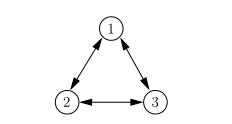
\includegraphics[width=0.49\linewidth]{3.png}
				\captionof{figure}{A graph of 3 nodes} 
			\end{center}
			 
			In \cite{bib13}, a class of randomized algorithms called \textit{quantized gossip algorithms} is proposed; see also \cite{bib06}. The following are the requirements for such algorithms: At time $k$, one edge  $\left\{ i, j \right\} \in \varepsilon$  is selected at random in an i.i.d. fashion. Let  $D_{ij}(k)=\left| x_{i}(k)-x_{j}(k) \right|$.  
			\begin{enumerate}[label=(\alph*)] 	
				\item If $D_{ij}(k)=0$, then the values of the nodes $i$ and $j$ remain the same for time $k+1$. \item If $D_{ij}(k)=1$, then the values are exchanged, or \textit{swapped}, by 	
				\begin{equation} 		
					x_{i}(k+1)=x_(j)(k) \text{ and } x_{j}(k+1)=x_{i}(k). 	
				\end{equation} 	
				\item Otherwise, the updates in the values satisfy 	
				\begin{equation*} 		
					x_{i}(k+1)+x_{j}(k+1)=x_{i}(k)+x_{j}(k), 	
				\end{equation*} 	
				\begin{equation*} 		
					D_{ij}(k+1)< D_{ij}(k). 	
				\end{equation*} 
			\end{enumerate} 
			Notice that algorithms in this class are by definition randomized. One way of specifying the distribution for choosing the edges is to allocate positive probabilities to all edges in the graph. We refer the readers to \cite{bib13} for several explicit quantized gossip algorithms that ensure the requirements above. We also emphasize that these algorithms are different from the one for the real-valued case in Section VB. Especially, the swapping in (7) become crucial when the node values are close to the average.   The next result applies to any such algorithm \cite{bib13}. \textit{Theorem 2:} For each initial condition $x(0)\in \mathbb{Z}^{\mathrm{N}}$, a quantized gossip algorithm achieves quantized average consensus in a finite number of steps with probability one.  An interesting aspect of this algorithm is that randomization is essential. This can be illustrated through an example given in \cite{bib13}.  Consider the graph with three nodes in Fig. 3. Initially, the node is given the value $i$ for $i = 1, 2, 3$ and, thus, the average value is $2$.  Suppose that we employ a deterministic, periodic scheme for the edge selection with period 3 by following $\left\{ 1, 2 \right\}, \left\{ 1, 3 \right\}, \left\{ 3, 2 \right\}, \left\{ 1, 2 \right\}, \ldots$. Under this scheme, it is clear that only swapping in (7) will take place for all times. Hence, the set of node values remains $1$, $2$, and $3$ and will never reach the consensus values. In contrast, by randomly choosing the edges, average consensus is possible in a matter of a few steps. This is an attractive communication scheme for its simplicity.  We remark that in \cite{bib13} further probabilistic analysis is given on the expected running time for achieving quantized consensus. In particular, if the graph is either fully connected or linear (i.e., the nodes are connected as $1$ – $2$ – $\cdots$ – $N$), then the expected running time is polynomial with respect to the number of nodes. Hence, this algorithm is an example of an efficient Las Vegas algorithm. This is in contrast with the real valued case in Section V-B, where in general convergence of the node values to the average is guaranteed only asymptotically.  
			 
			\subsection{\textit{Binary-valued case}}
			The third consensus problem we study is when the agents take binary values $x_{i}(k) 
			\in \left\{ 0,1 \right\}$ for all $i, k$. In particular, the problem we discuss here is known as the 
			\textit{Byzantine 	agreement} problem in the field of distributed computing, see e.g. \cite{bib17}. We will show that in this case even stronger results in favor of randomized schemes can be obtained.  A distinct feature of this problem is that some of the $N$ agents are faulty. Such agents may try to deceive the nonfaulty agents and may even communicate to each other secretly. We assume that there are $N_{f}$ such agents, which are fixed but their identity is not known to the nonfaulty ones. Regarding the communication pattern, the graph is fully connected. Each agent sends a message to all others at each time $k$; faulty agents may send different messages to others. Randomization hence takes part not in the communication pattern. Instead, a \textit{global coin toss} is performed by a trusted party who sends the (true) result to all agents at each $k$.  The objective is to achieve a form of average consensus even in the worst case. We say that \textit{binary consensus} is achieved if each agent $i$ determines the \textit{decision value} $y_{i} \in \left\{ 0,1 \right\}$ such that 
			\begin{enumerate}[label=(\roman*)] 	
				\item all nonfaulty agents arrive at the same decision value; 	 	
				\item if all nonfaulty agents have the same initial value 	$x_{i}(0)$, then they finish with $y_{i} = x_{i}(0)$. 
			\end{enumerate}  
				We consider the simple case where $N$ is a multiple of $8$ and $N_{f} < N/8$. We also let 
			\begin{equation*} 	
				L:=5N/8+1,\; H:=3N/4+1,\; G:=7N/8. 
			\end{equation*}  
			The algorithm for each agent i we now present is due to \cite{bib19}; basically, the agent sends its value and decides on the majority of the values that it receives. 
			\begin{center}
				\begin{tabular}{||c||} 
					\hline
					1) \, At time $k$, send the value $x_{i}(k)$ to other agents and \\
					receive $x_{j}(k), \; j\neq i$, from them.\\ [0.5ex] 
					\hline
					2) \, Set the \textit{majority value} $m_{i}(k)\in \left\{ 0,1 \right\}$ \\
					to what the
					majority of agents sent as their values. Then, set the\\
					\textit{tally} $t_{i}(k)$ equal to the number of agents whose values\\
					are the same as $m_{i}(k)$.\\ 
					\hline
					3) \, Now, depending on the result of the coin toss, let the\\
					\textit{threshold} $\overline{t}(k)$ be $L$ if the coin shows
					heads and $H$\\
					otherwise (note that the threshold is the same for all
					agents).\\
					\hline
					4) \, Set the value $x_{i}(k)$ to the majority value $m_{i}(k)$ if\\
					$t_{i}(k) \ge \overline{t}(k)$ and to 0 otherwise.\\
					\hline
					5) \, If the tally satisfies $t_{i}(k) \ge G$, then let the decision\\
					value $y_{i}$ be equal to $m_{i}(k)$.\\
					\hline
				\end{tabular}
			\end{center}
			\begin{comment}
				\begin{enumerate}[label=\arabic*)] 	
					\item At time $k$, send the value $x_{i}(k)$ to other agents and receive $x_{j}(k),\; j\neq i$, from them. 	 	
					\item Set the \textit{majority value} $m_{i}(k)\in \left\{ 0,1 \right\}$ to what the majority of agents sent as their values. Then, set the \textit{tally} $t_{i}(k)$ equal to the number of agents whose values 	are the same as $m_{i}(k)$. 	 	
					\item Now, depending on the result of the coin toss, let the \textit{threshold} $\overline{t}(k)$ be $L$ if the coin shows heads and $H$ 	otherwise (note that the threshold is the same for all 	agents). 	 	
					\item Set the value $x_{i}(k)$ to the majority value $m_{i}(k)$ if 	$t_{i}(k) 
					\ge 
					\overline{t}(k)$ and to 0 otherwise. 	 	
					\item If the tally satisfies $t_{i}(k) 
					\ge G$, then let the decision 	value $y_{i}$ be equal to $m_{i}(k)$. 
				\end{enumerate}
			\end{comment}  
			There are two simple situations. (a) When all nonfaulty agents have the same value at one point, all of them will finish with this value as their decision values in a constant number of steps. (b) When two nonfaulty agents have different majority values; then, all values $x_{i}(k)$ will become $0$ during this step because none of the tallies exceeds the threshold (in step 4 above).  The interesting case is when all nonfaulty agents have the same majority value. Then, the faulty agents have a chance to confuse them. This can be done by making some nonfaulty agents have tallies exceeding the threshold and others have tallies smaller than the threshold. However, under the scheme, the chance is limited. Since $H−L \ge N_{f}$ , the faulty agents can deceive any agent only for one of the threshold values, $L$ or $H$. Further, the threshold randomly varies over $L$ and $H$ because of the coin toss. Consequently, the probability of deceiving is $1/2$. On the other hand, when they fail to deceive, all nonfaulty agents take the same value, which leads to consensus.  The main result concerning the Byzantine agreement problem is given below \cite{bib17}. \textit{Theorem 3:} For the algorithm presented above, binary consensus is achieved with probability one for each initial condition $x(0) \in \left\{ 0,1 \right\}^{N}$. Moreover, the expected number of steps required is a constant.  This theorem implies that the consensus algorithm is an efficient Las Vegas type. In contrast, it is known that any deterministic algorithm requires $N_{f}+1$ steps \cite{bib17}. It is emphasized that even stronger results have been obtained in the area of distributed computing. One is the so-called \textit{impossible result} for an asynchronous version of the binary consensus problem \cite{bib09}. This result states that if there is no synchronized clock owned by the agents and if there is no assumption on the sampling periods of the agents (i.e., the processing speed may be different), for any deterministic algorithm, it is impossible to achieve consensus. Randomized schemes such as using a global coin toss have been shown to be effective in this case as well. For a survey on this topic, which also includes many recent improvements on the original algorithm, we refer to \cite{bib02}.  
			
		
		\section{CONCLUSION}
		In this paper, we discussed several variations of the average consensus problem and the role of probabilistic algorithms in this context. The class of Las Vegas randomized algorithms, which has been recently employed in the field of systems and control \cite{bib11}, \cite{bib24}, has been shown to be effective and sometimes crucial. Future research will deal with other consensus problems where the agents take real/quantized values and may be faulty.
		\textit{Acknowledgment}: The authors would like to thank Teodoro Alamo, Tamer Bas¸ar, Ivan Cibrario Bertolotti, Yasumasa Fujisaki, Akshay Kashyap, and Sandro Zampieri for the interesting discussions and for the valuable comments.
		
% End Fateme's part__________________________________________________________
	
	
	\begin{thebibliography}{30}
		
		\bibitem{bib01} P. J. Antsaklis and J. Baillieul, Guest Editors. Special Issue on the Technology of Networked Control Systems.\textit{Proc. IEEE,} 95(1), 2007.
		
		
		\bibitem{bib02} J. Aspnes. Randomized protocols for asynchronous consensus. \textit{Distributed Computing}, 16:165–175, 2003.
		
		
		\bibitem{bib03} D. P. Bertsekas and J. N. Tsitsiklis.\textit{Parallel and Distributed Computation: Numerical Methods.} Prentice-Hall, Englewood Cliffs, NJ,1989.
		
		
		\bibitem{bib04} D. P. Bertsekas and J. N. Tsitsiklis. Comments on “Coordination of groups of mobile autonomous agents using nearest neighbor rules”. \textit{IEEE Trans. Autom. Control,} 52:968–969, 2007.
		
		
		\bibitem{bib05} V. D. Blondel, J. M. Hendrickx, A. Olshevsky, and J. N. Tsitsiklis. Convergence in multiagent coordination, consensus, and flocking. In \textit{Proc. 44th IEEE Conf. on Decision and Control and European Control Conf.,} pages 2996–3000, 2005.
		
		
		\bibitem{bib06} S. Boyd, A. Ghosh, B. Prabhakar, and D. Shah. Randomized gossip algorithms. \textit{IEEE Trans. Information Theory}, 52:2508–2530, 2006.
		
		
		\bibitem{bib07} R. Carli, F. Fagnani, M. Focoso, A. Speranzon, and S. Zampieri. Communication constraints in the average consensus problem. \textit{Automatica,} 44:671–684, 2008.
		
		
		\bibitem{bib08} M. Deng and Y.-C. Ho. An ordinal optimization approach to optimal control problems. \textit{ Automatica,} 35:331–338, 1999.
		
		
		\bibitem{bib09} M. J. Fisher, N. A. Lynch, and M. S. Paterson. Impossibility of distributed consensus with one faulty processor. \textit{J. ACM}, 32:374–382, 1985.
		
		
		\bibitem{bib10} Y. Hatano and M. Mesbahi. Agreement over random networks. \textit{IEEE Trans. Autom. Control,} 50:1867–72, 2005.
		
		
		\bibitem{bib11} H. Ishii and R. Tempo. Probabilistic sorting and stabilization of switched systems. Submitted for publication, 2007.
		
		
		\bibitem{bib12} A. Jadbabaie, J. Lin, and A. S. Morse. Coordination of groups of mobile autonomous agents using nearest neighbor rules. \textit{IEEE Trans. Autom. Control}, 48:988–1001, 2003.
		
		
		\bibitem{bib13} A. Kashyap, T. Bas¸ar, and R. Srikant. Quantized consensus. \textit{Automatica}, 43:1192–1203, 2007.
		
		
		\bibitem{bib14} D. E. Knuth. \textit{The Art of Computer Programming,} 2nd edition, volume 3: Sorting and Searching. Addison-Wesley, Reading, MA, 1998.
		
		
		\bibitem{bib15} M. Mitzenmacher and E. Upfal. \textit{Probability and Computing: Randomized Algorithms and Probabilistic Analysis.} Cambridge University Press, 2005.
		
		
		\bibitem{bib16} L. Moreau.Stability of multiagent systems with time-dependent communication links.\textit{IEEE Trans. Autom. Control}, 50:169–182,2005.
		
		
		\bibitem{bib17} R. Motwani and P. Raghavan. \textit{Randomized Algorithms}. Cambridge University Press, 1995.
		
		
		\bibitem{bib18} R. Olfati-Saber and R. Murray. Consensus problems in networks of agents with switching topology and time-delays. \textit{IEEE Trans. Autom. Control,} 49:1520–1533, 2004.
		
		
		\bibitem{bib19} M. O. Rabin. Randomized Byzantin generals. In \textit{Proc. Annual Symp. on Foundations of Computer Science}, pages 403–409, 1983.
		
		
		\bibitem{bib20} A. V. Savkin. Coordinated collective motion of groups of autonomous robots: Analysis of Vicsek’s model. \textit{IEEE Trans. Autom. Control,}49:981–983, 2004.
		
		
		\bibitem{bib21} A. Tahbaz-Salehi and A. Jadbabaie. Necessary and sufficient conditions for consensus over random independent and identically distributed switching graphs. In \textit{Proc. 46th IEEE Conf. on Decision and Control,} pages 4209–4214, 2007.
		
		
		\bibitem{bib22} R. Tempo, E. W. Bai, and F. Dabbene. Probabilistic robustness analysis: Explicit bounds for the minimum number of samples. \textit{Systems and Control Letters}, 30:237–242, 1997.
		
		
		\bibitem{bib23}  R. Tempo, G. Calafiore, and F. Dabbene. \textit{Randomized Algorithms for Analysis and Control of Uncertain Systems.} Springer, London, 2005.
		
		
		\bibitem{bib24} R. Tempo and H. Ishii. Monte Carlo and Las Vegas randomized algorithms for systems and control: An introduction. European J. Control, 13:189–203, 2007.
		
		
		\bibitem{bib25} J. N. Tsitsiklis. \textit{Problems in Decentralized Decision Making and Computation}. PhD thesis, Dept. of Electrical Engineering and Computer Science, MIT, 1984. \href{http://web.mit.edu/jnt/www/Papers/PhD-84-jnt.pdf.}{http://web.mit.edu/jnt/www/Papers/PhD-84-jnt.pdf.}
		
		
		\bibitem{bib26} M. Vidyasagar. Statistical learning theory and randomized algorithms for control. \textit{IEEE Control Systems Magazine,} 18(6):69–85, 1998
		
		
		\bibitem{bib27} C. W. Wu. Synchronization and convergence of linear dynamics in random directed networks. \textit{IEEE Trans. Autom. Control,} 51:1207–1210, 2006.
		
		
		\bibitem{bib28} L. Xiao, S. Boyd, and S. Lall. A scheme for robust distributed sensor fusion based on average consensus. In \textit{Proc. Conf. on Information Processing in Sensor Networks,} pages 63–70, 2005.
		
	\end{thebibliography}
	
	
\end{document}
